%%%%%%%%%%%%%%%%%%%%%%%%%%%%%%%%%%%%%%%%%%%%%%%%%%%%%%%%%%%%%%%%%%%%%
%
%  This is a sample LaTeX input file for your contribution to
%  the M&C2023 topical meeting.
%
%  Please use it as a template for your full paper
%    Accompanying/related file(s) include:
%       1. Document class/format file: mc2023.cls
%       2. Sample PDF/Postscript Figure: figure.pdf,figure.ps
%       3. A PDF file showing the desired appearance: mc2023_template.pdf
%       4. cites.sty and citesort.sty that might be needed by some users
%    Direct questions about these files to: buijsa@mcmaster.ca
%    Originals provided by brantley1@llnl.gov
%
%    Notes:
%      (1) You can use the "dvips" utility to convert .dvi
%          files to PostScript.  Then, use either Acrobat
%          Distiller or "ps2pdf" to convert to PDF format.
%      (2) Different versions of LaTeX have been observed to
%          shift the page down, causing improper margins.
%          If this occurs, adjust the "topmargin" value in the
%          mc2023.cls file to achieve the proper margins.
%
%%%%%%%%%%%%%%%%%%%%%%%%%%%%%%%%%%%%%%%%%%%%%%%%%%%%%%%%%%%%%%%%%%%%%


%%%%%%%%%%%%%%%%%%%%%%%%%%%%%%%%%%%%%%%%%%%%%%%%%%%%%%%%%%%%%%%%%%%%%
\documentclass[letterpaper]{mc2023}
%
%  various packages that you may wish to activate for usage
\usepackage{tabls}
\usepackage{cites}
\usepackage{epsf}
\usepackage{appendix}
\usepackage{ragged2e}
\usepackage[top=1in, bottom=1in, left=1in, right=1in]{geometry}
\usepackage{enumitem}
\setlist[itemize]{leftmargin=*}
\usepackage{caption}
\captionsetup{width=1.0\textwidth,font={bf,normalsize},skip=0.3cm,within=none,justification=centering}

\usepackage[justification=centering]{caption}

% ELIMINATING WHITESPACE
\setlength{\belowcaptionskip}{-15pt}
\setlength{\abovedisplayskip}{4pt}
\setlength{\belowdisplayskip}{4pt}


\usepackage{xcolor}
\usepackage[colorlinks = true, linkcolor = black, urlcolor  = black, citecolor = black]{hyperref}
\usepackage{float} % for [H] option in figures

% GLOSSARIES
\usepackage[acronym,nomain,nonumberlist,nogroupskip,nopostdot]{glossaries} % for glossary of acronyms
\usepackage{siunitx}
\setacronymstyle{long-short}
\loadglsentries{glossary}
\makeglossaries
\renewcommand*{\glstextformat}[1]{\textcolor{black}{#1}} % make glossary color black

% Lewis custom commands
% This file contains custom commands that Lewis uses frequently in LaTeX documents

\usepackage{subcaption}
\usepackage{hyperref}
\hypersetup{colorlinks,allcolors=black}
% for more https://tex.stackexchange.com/questions/88400/hyperref-changing-the-linkcolor-locally-in-the-toc
\usepackage{amssymb}
\usepackage{bbm}

% matlab stuff
\usepackage{graphicx}
\usepackage{color}
\usepackage{matlab-prettifier}

%vector arrow
\usepackage{graphicx}
\newcommand{\cev}[1]{\reflectbox{\ensuremath{\vec{\reflectbox{\ensuremath{#1}}}}}}
% table packages
\usepackage{booktabs}
\usepackage{adjustbox}

% custom equation commands
\newcommand{\QOR}{\qquad \text{OR} \qquad}
\newcommand{\QAND}{\qquad \text{AND} \qquad}
\newcommand{\QTHUS}{\qquad \text{THUS} \qquad}
\newcommand{\QWITH}{\qquad \text{WITH} \qquad}
\newcommand{\QFOR}{\qquad \text{FOR} \qquad}
\newcommand{\QSO}{\qquad \text{SO} \qquad}
\newcommand{\QWHERE}{\qquad \text{WHERE} \qquad}
\newcommand{\QWHEN}{\qquad \text{WHEN} \qquad}
\newcommand{\LINE}{\par\noindent\rule{\textwidth}{0.4pt}\par}
\newcommand{\toinf}{\rightarrow\infty}
\newcommand{\tozero}{\rightarrow0}
\newcommand{\qeq}{\overset{?}{=}}
\newcommand{\ceq}{\overset{\checkmark}{=}}
\newcommand{\Poi}{\text{Poisson}}
\newcommand{\keff}{$k_{e\!f\!f}$}
\renewcommand{\epsilon}{\varepsilon} % squiggly epsilon

\def\brac#1{\{#1\}}
\def\Brac#1{\big\{#1\big\}}
\def\BRAC#1{\bigg\{#1\bigg\}}
\def\angbrac#1{\langle#1\rangle}
\def\Angbrac#1{\big\langle#1\big\rangle}
\def\ANGBRAC#1{\bigg\langle#1\bigg\rangle}
\usepackage{float}
% SI Units
\usepackage{siunitx}
\DeclareSIUnit\n{n}
\DeclareSIUnit\sp{sp}

\def\doubleunderline#1{\underline{\underline{#1}}}

\title{Verification of the Cardinal Multiphysics Solver for 1-D Coupled\\
Heat Transfer and Neutron Transport}

\author{%
  % FIRST AUTHORS
  %
  \textbf{L.I.~Gross$^1$, A.J.~Novak$^2$, P.Shriwise$^2$, and P.P.H.~Wilson$^1$}\\
  $^1$University of Wisconsin -- Madison  \\
  1500 Engineering Drive, Madison, WI 53706 \vspace{6pt}\\
  $^2$Argonne National Laboratory \\
  9700 S Cass Avenue, Lemont, IL 60439\vspace{6pt} \\
  \url{ligross@wisc.edu}, \url{anovak@anl.gov}, \url{pshriwise@anl.gov} \url{paul.wilson@wisc.edu}
}
%
% Insert authors' names and short version of title in lines below
%
\newcommand{\authorHead}{Gross et al.}
\newcommand{\shortTitle}{Cardinal Multiphysics Analytical Benchmark Verification}
%
%%%%%%%%%%%%%%%%%%%%%%%%%%%%%%%%%%%%%%%%%%%%%%%%%%%%%%%%%%%%%%%%%%%%%
%
%   BEGIN DOCUMENT
%
%%%%%%%%%%%%%%%%%%%%%%%%%%%%%%%%%%%%%%%%%%%%%%%%%%%%%%%%%%%%%%%%%%%%%
\begin{document}
\maketitle
\justify
\parskip 6pt plus 1 pt minus 1 pt

\begin{abstract}
  Cardinal is a multiphysics software tool that couples OpenMC Monte Carlo transport and NekRS \gls{cfd} to the \gls{moose}.
  In this work, we verify Cardinal for coupled heat conduction and neutron transport using a 1-D analytic solution from previous
  work by the Naval Nuclear Laboratories. This numerical benchmark includes $S_2$ transport, Doppler-broadened cross-sections,
  thermal conduction and expansion, and convective boundary conditions. The goals of this work are to verify Cardinal's basic
  multiphysics modeling capabilities for coupled neutronics and heat conduction, while serving as a computational ``test bed''
  for assessing the performance of various multiphysics coupling strategies and algorithms.
  \begin{itemize}
      \item Temperature and flux distributions match.
      \item Error study convergence, report slope aka first order
  \end{itemize}
\end{abstract}
\vspace{6pt}
\keywords{Cardinal, MOOSE, OpenMC, multiphysics, verification}

\section{INTRODUCTION}
\label{sec:intro}
With recent advancements in methods, software, and computing, high-fidelity multiphysics \gls{ms} is becoming an important
component of the nuclear engineer's ``toolbox.'' These high-fidelity models substitute excessively pessimistic safety factors
with predictive science. This can reduce uncertainty in analyses, enabling tighter margins to realize improved economics
and licensing certainty. However, analytical benchmarks and comparison to experimental data are required to assess the stability,
convergence, and predictive capability of these high-fidelity models for reactor design and analysis.

Cardinal \cite{novak2022_cardinal} is an open-source code  that couples OpenMC \cite{openmc} Monte Carlo particle transport and
NekRS \gls{cfd} to \gls{moose} \cite{lindsay2022moose}. This coupling brings high-fidelity multiphysics feedback to the \gls{moose}
``ecosystem.'' Cardinal couples OpenMC and NekRS to \gls{moose} simulations by copying data between the internal code data structures
(e.g. a vector of tally results in OpenMC) and a \texttt{MooseMesh}, or the unstructured mesh class in \gls{moose}. \gls{moose}'s
mesh-to-mesh interpolation system then communicates between the \texttt{MooseMesh} ``mirror'' of the external code's solution and an
arbitrary coupled \gls{moose} application in the form of boundary conditions (such as for conjugate heat transfer with NekRS) or
source terms (such as for volumetric heating with OpenMC). Convergence is obtained with Picard iteration.

For coupled neutronics-thermal-fluid simulations with OpenMC, each Picard iteration consists of several steps: 1)~a \gls{moose}
application (e.g. BISON, Pronghorn, NekRS via Cardinal, ...) solves for temperatures and densities; 2)~Cardinal transfers
temperatures and densities to the OpenMC model; 3)~OpenMC solves for the nuclear heating; and 4)~Cardinal transfers the tally
values to the \texttt{MooseMesh} ``mirror.''

These steps continue until convergence criteria is achieved. In this work, we pursue verification of these multiphysics aspects
of Cardinal using a 1-D analytical benchmark from the Naval Nuclear Laboratories \cite{analytical_benchmark}.  This work does
not require \gls{cfd}, and thus NekRS will be left out of discussion from this point on.

The remainder of this paper is organized as follows. In Section \ref{sec:benchmark}, we summarize the analytical benchmark
modeled in this work. Section \ref{sec:model} then describes the Cardinal computational model of the benchmark. Section
\ref{sec:results} presents comparisons between Cardinal and the analytical benchmark. Finally, Section \ref{sec:conclusions}
presents conclusions and outlines ongoing and future efforts in the verification and validation of Cardinal.

\section{BENCHMARK PROBLEM DESCRIPTION}
\label{sec:benchmark}
The analytical benchmark is a coupling between three physics: $S_2$ neutron transport (with Doppler broadening), heat conduction,
and thermal expansion. $S_{2}$ transport restricts the neutron direction to only the $\pm x$ direction. A summary of the governing
equations and boundary conditions in the 1-D slab is shown in Fig. \ref{fig:slab_diagram}.
\begin{figure}[H]
    \centering
    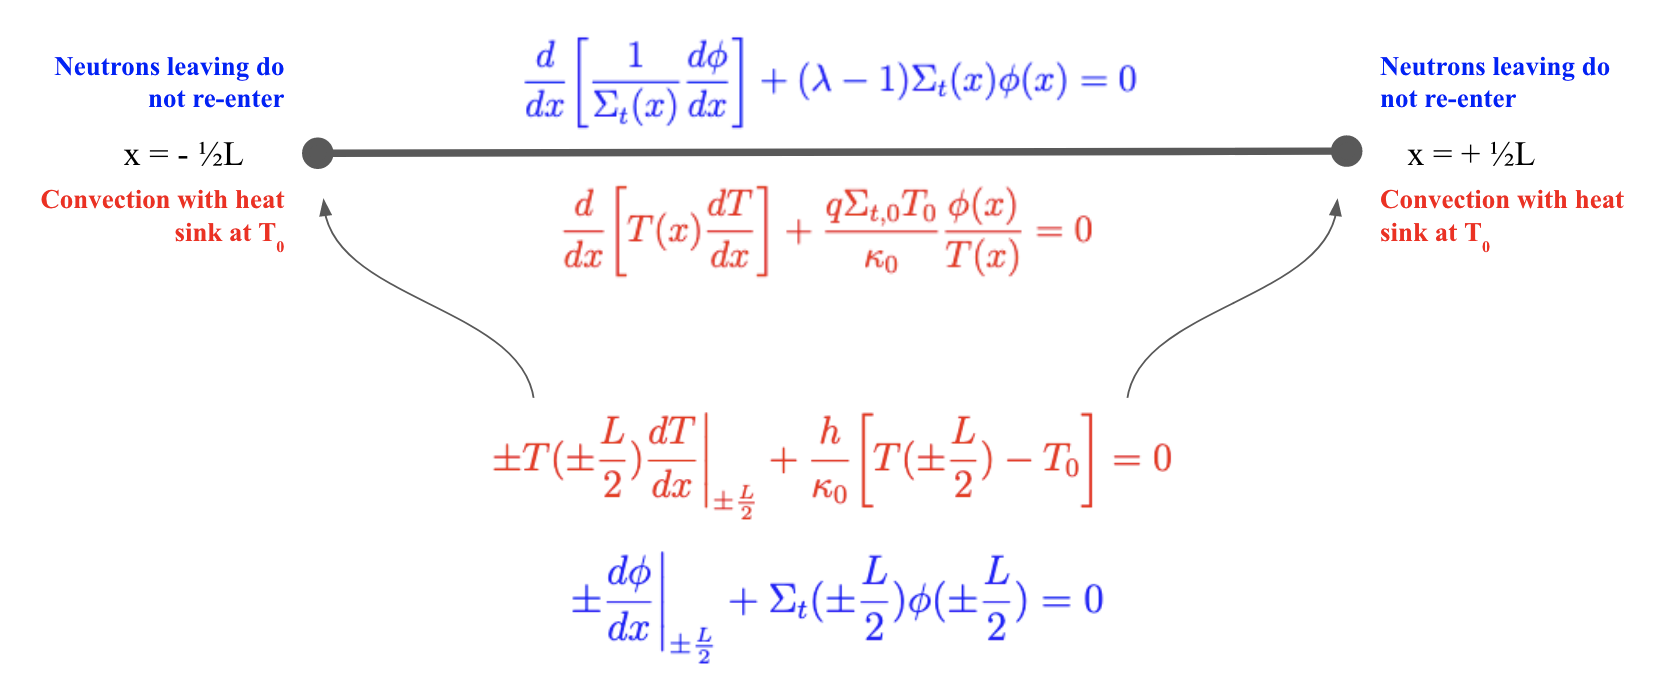
\includegraphics[width=0.55\linewidth]{figures/1D_Benchmark_Diagram.png}
    \caption{This diagram summarizes the domain, governing ODEs, and boundary conditions for the slab.}
    \label{fig:slab_diagram}
\end{figure}

This benchmark uses a one-group assumption for the neutron cross-sections. As neutrons transport, fission events deposit volumetric
power in the form of heat in the slab, causing thermal expansion and affecting the temperature distribution. In this benchmark,
thermal expansion is restricted to only the $x$-direction. This slab elongation feeds back neutronics and heat conduction by
influencing the domain length and material density. The slab has convective boundary conditions at the endpoints $x=\pm \frac{L}{2}$
with the heat sink temperature $T_{0}$. The Doppler-broadened total microscopic cross-section follows an inverse-root temperature
relationship,
\begin{equation}
    \sigma_{t}(T) = \sigma_{t,0}\sqrt{\frac{T_{0}}{T(x)}}
\end{equation}
Due to thermal expansion, the slab density varies as
\begin{equation} \label{sec:intro:density}
    \rho(x) =  \rho_{0} \sqrt{\frac{T_{0}}{T(x)}},
\end{equation}
This gives a Doppler-broadened, macroscopic total cross-section that accounts for changes in density due to temperature as
\begin{equation} \label{sec:intro:doppler}
    \Sigma_{t}(x) = \frac{\rho_{0}\sigma_{t,0} N_{A}}{A} \frac{T_{0}}{T(x)} = \Sigma_{t,0}\frac{T_{0}}{T(x)} ,
\end{equation}
where $ \sigma_{t,0}$ is the total microscopic cross-section at $T_{0}$, $N_{A}$ is Avogadro's number, and $A$ is the mass number
of the medium. The conduction equation governs heat flow in the slab and can be described in terms of the thermal conductivity
$\kappa(T)$,the energy released per fission $q$, the total macroscopic cross-section $\Sigma_{t}$, and the neutron flux $\phi$.
\begin{equation}
     \frac{d}{dx}\bigg[\kappa(T(x))\frac{dT(x)}{dx}\bigg] + q \Sigma_{t}(x)\phi(x) = 0.
\end{equation}
The main assumption used to craft the analytical solution is that $T(x)=f\phi(x)$. This assumption is held up by manipulating
the differential equations, inserting the cross-section temperature dependence, and matching coefficients so that the two ODEs
are of the same solution type. The matching of coefficients imposes two constraints that give equations for the total microscopic
cross-section $\sigma_{t,0}$ and the heat transfer coefficient $h$ in terms of the slab parameters. These are two key parameters
required as inputs for the simulation. For full details on the analytical solution's derivation, see \cite{analytical_benchmark}.


\section{COMPUTATIONAL MODEL}
\label{sec:model}
This section describes the OpenMC and \gls{moose} computational models, followed by the convergence criteria used for coupling.
Note that Cardinal currently does not yet support moving geometries in OpenMC. Instead, the simulation uses the formula for
equilibrium length $L$ from \cite{analytical_benchmark} that accounts for all three physics effects. The change in density due
to temperature is accounted for by using the total macroscopic cross-section\ --\ which has a density factor\ --\ from
(\ref{sec:intro:doppler}), as was mentioned in Section \ref{sec:benchmark}.

\subsection{OpenMC Model}
The geometry used in OpenMC must be finite, despite the benchmark being infinite in the $y$ and $z$ directions. In general,
reflective boundary conditions can be used to simulate infinite dimensions. Thus, this benchmark can be represented with
vacuum boundary conditions at $x=\pm \frac{L}{2}$ and reflective boundary conditions at the $y$ and $z$ boundaries. Fig.
\ref{fig:slab_diagram} showed a diagram of the geometry, governing equations, and boundary conditions for the different physics.

The benchmark's one-group assumption was satisfied using OpenMC's multigroup mode, as opposed to typical continuous energy
transport. OpenMC allows user-defined cross-sections with the \texttt{XSdata} class. The cross-section for each reaction was
specified at an array of temperatures and was exported to a library allowing a look-up or interpolation to determine the
cross-section in each region as temperature changes during iteration.

The OpenMC model required slight source code modifications to accommodate $S_2$-like transport. In typical OpenMC simulations,
the physics of each reaction describes the scattering dynamics. The Monte Carlo algorithm is agnostic to the direction
particles move, but it is not typically constrained to a discrete directional distribution. However, when modeling this
benchmark, any history with a particle moving perpendicular to the $x$-direction would attenuate particles in less
$x$-distance than if particles were constrained to either $\pm x$. To address this, we first use OpenMC's \texttt{PolarAzimuthal}
distribution to restrict the birth direction of particles to the $\pm x$ direction. We then also modified OpenMC in a
patched branch to mimic $S_{2}$ transport in two ways. First, when determining the angular cosine of scattering events,
$\mu$, particles either continue forward ($\mu=1$) or are back-scattered ($\mu=-1$) with equal probability, as opposed to
sampling the reaction physics for $\mu$. Second, since the simulation uses $k$-eigenvalue mode, neutrons born in subsequent
generations of the simulation also need to have their angular distributions restricted to $\pm x$. \textbf{Additional details on
the OpenMC model will be presented in the full paper.}

\subsection{MOOSE Heat Conduction Model}
The \gls{moose} heat conduction module is used to solve for thermal heat conduction with convection boundary conditions.
\textbf{TODO Additional details on the MOOSE model will be presented in the full paper.}
\textbf{TODO describe heat conduction model in more depth}
\subsection{Convergence Criteria}
There are two types of convergence criteria used in this benchmark. The first type of convergence criteria relates to the
constituent iterations of single physics solves: neutronics and heat conduction. Monte Carlo is not an iterative method,
so batching settings are required before the simulation. The k-eigenvalue simulation used 50,000 particles per batch,
with 50 inactive batches and 50 active batches for every case. Additionally, the Robbins-Monro relaxation also contributed
to increasing the number of histories included in the flux statistics. While flux is typically reported with an uncertainty,
Cardinal does not currently support computing the uncertainty for cases using relaxation; though, an analytical solution for
flux is given. With this, the true error can be computed, as opposed to a statistical uncertainty which is typically reported.
The heat conduction, however, relies on MOOSE's iterative FEM solver. The convergence criteria for heat conduction is given by
\begin{lstlisting}
  nl_abs_tol = 1e-7
  nl_rel_tol = 1e-9
  petsc_options_iname = '-pc_type -pc_hypre_type'
  petsc_options_value = 'hypre boomeramg'
\end{lstlisting}

The second type of convergence relates to global iterations, i.e. Picard Iterations. Since this is a steady-state problem being
run with a transient solver, MOOSE's steady state detection feature was turned on. The steady state tolerance selected was $1e-5$.
\textbf{explain how the SS tolerance works i.e. L2 norm. Discuss what was included}. This led to increasing number of iterations
to achieve steady state as the mesh refined. Below is a figure showing this relationship.

% \begin{figure}[H]
%     \centering
%     \includegraphics{}
%     \caption{Caption}
%     \label{fig:my_label}
% \end{figure}

\section{RESULTS}\label{sec:results}

\begin{itemize}
    \item TODO add error plot
    \item TODO add temperature plot
    \item TODO add flux for finest mesh size
\end{itemize}
\section{CONCLUSIONS}\label{sec:conclusions}

\begin{itemize}
    \item TODO comment on error trend.
    \item TODO comment on temperature and flux distributions matching well.
\end{itemize}


\section{CONCLUSIONS}


\section*{NOMENCLATURE}

% TODO fix glossary
\printglossary[title={Nomenclature}, nonumberlist, nopostdot]

\section*{ACKNOWLEDGEMENTS}
The authors would like to thank the OpenMC and MOOSE development teams for their guidance in model setup and assistance
with software. We also want to thank Dr. Griesheimer and Dr. Kooreman for their modeling advice and knowledge about the
analytical benchmark.

\setlength{\baselineskip}{12pt}
\bibliographystyle{mc2023}
\bibliography{mc2023}
\setlength{\baselineskip}{12pt}


\end{document}
